\documentclass[a4paper,12pt]{article}

% Packages for math, formatting, and images
\usepackage[utf8]{inputenc}
\usepackage{amsmath, amssymb, amsthm}
\usepackage{geometry}
\usepackage{graphicx}
\usepackage{listings}
\usepackage{xcolor}
\usepackage{hyperref}

\geometry{margin=1in}

% Code listing style
\definecolor{codegreen}{rgb}{0,0.6,0}
\definecolor{codegray}{rgb}{0.5,0.5,0.5}
\definecolor{codepurple}{rgb}{0.58,0,0.82}
\definecolor{backcolour}{rgb}{0.95,0.95,0.92}

\lstdefinestyle{mystyle}{
    backgroundcolor=\color{backcolour},   
    commentstyle=\color{codegreen},
    keywordstyle=\color{magenta},
    numberstyle=\tiny\color{codegray},
    stringstyle=\color{codepurple},
    basicstyle=\ttfamily\footnotesize,
    breakatwhitespace=false,         
    breaklines=true,                 
    captionpos=b,                    
    keepspaces=true,                 
    numbers=left,                    
    numbersep=5pt,                  
    showspaces=false,                
    showstringspaces=false,
    showtabs=false,                  
    tabsize=2
}
\lstset{style=mystyle}

\title{ES 446: Assignment 4 \\ \large Reaction-Diffusion Equation Implementation in FEniCS}
\author{Assignment Report}
\date{\today}

\begin{document}

\maketitle

\section{Introduction}
The objective of this assignment is to implement the Reaction-Diffusion equation on a unit square domain $\Omega = [0, 1] \times [0, 1]$. We utilize the FEniCS finite element computing platform to solve the resulting partial differential equation (PDE) over time.

\section{Problem Statement}
The governing strong form of the reaction-diffusion equation is given by:
\begin{equation}
    \frac{\partial u}{\partial t} = D \nabla^2 u + f(u) \quad \text{in } \Omega
\end{equation}
where:
\begin{itemize}
    \item $u(x, y, t)$ is the concentration variable.
    \item $D$ is the diffusion coefficient.
    \item $f(u) = \rho u(1 - u)$ is the reaction term (Fisher-KPP).
\end{itemize}

The boundary conditions are set as homogeneous Dirichlet:
\begin{equation}
    u = 0 \quad \text{on } \partial\Omega
\end{equation}

The initial condition is a Gaussian pulse centered in the domain:
\begin{equation}
    u(x, y, 0) = \exp\left(-100 \left[(x-0.5)^2 + (y-0.5)^2\right]\right)
\end{equation}

\section{Derivation of the Weak Formulation}
To solve the PDE using the Finite Element Method, we convert the strong form into its weak (variational) form.

\subsection{Time Discretization}
Using the Backward Euler method for the diffusion term and an explicit treatment for the reaction term (semi-implicit scheme):
\begin{equation}
    \frac{u^{n+1} - u^n}{\Delta t} - D \nabla^2 u^{n+1} = f(u^n)
\end{equation}

Rearranging for terms at time $t^{n+1}$:
\begin{equation}
    u^{n+1} - \Delta t D \nabla^2 u^{n+1} = u^n + \Delta t f(u^n)
\end{equation}

\subsection{Variational Form}
Multiply by a test function $v \in H_0^1(\Omega)$ and integrate over the domain $\Omega$:
\begin{equation}
    \int_\Omega u^{n+1} v \, dx - \Delta t D \int_\Omega (\nabla^2 u^{n+1}) v \, dx = \int_\Omega (u^n + \Delta t f(u^n)) v \, dx
\end{equation}

Applying Green's first identity to the Laplacian term:
\begin{equation}
    -\int_\Omega (\nabla^2 u^{n+1}) v \, dx = \int_\Omega \nabla u^{n+1} \cdot \nabla v \, dx - \int_{\partial \Omega} \frac{\partial u^{n+1}}{\partial n} v \, ds
\end{equation}

Since $v = 0$ on the boundary $\partial\Omega$ (Dirichlet BC), the boundary integral vanishes. The final weak form is: Find $u^{n+1} \in V$ such that for all $v \in V$:
\begin{equation}
    \int_\Omega (u^{n+1} v + \Delta t D \nabla u^{n+1} \cdot \nabla v) \, dx = \int_\Omega (u^n + \Delta t f(u^n)) v \, dx
\end{equation}

\section{Implementation}
The following Python code using FEniCS implements the derived variational problem.

\begin{lstlisting}[language=Python, caption=FEniCS Implementation]
# Bilinear form a(u, v) and linear form L(v)
a = (u * v + dt * D * dot(grad(u), grad(v))) * dx
L = (u_n + dt * rho * u_n * (1 - u_n)) * v * dx

# Time-stepping loop
while t < T:
    solve(a == L, u_sol, bc)
    u_n.assign(u_sol)
    t += dt
\end{lstlisting}

\section{Results}
The simulation results are captured in the plots below, showing the evolution from the initial Gaussian pulse to the diffused state.

\begin{figure}[h]
    \centering
    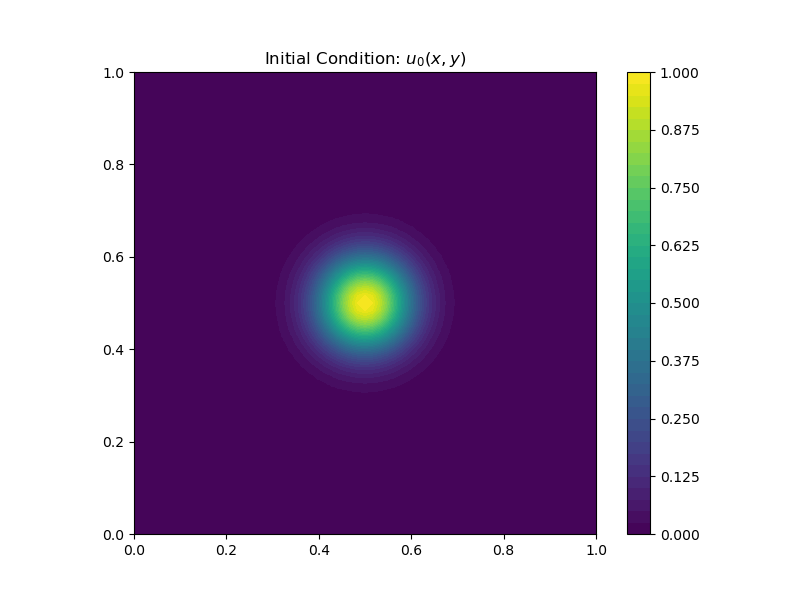
\includegraphics[width=0.7\textwidth]{initial_condition.png}
    \caption{Initial Condition: Gaussian Pulse}
    \label{fig:initial}
\end{figure}

\begin{figure}[h]
    \centering
    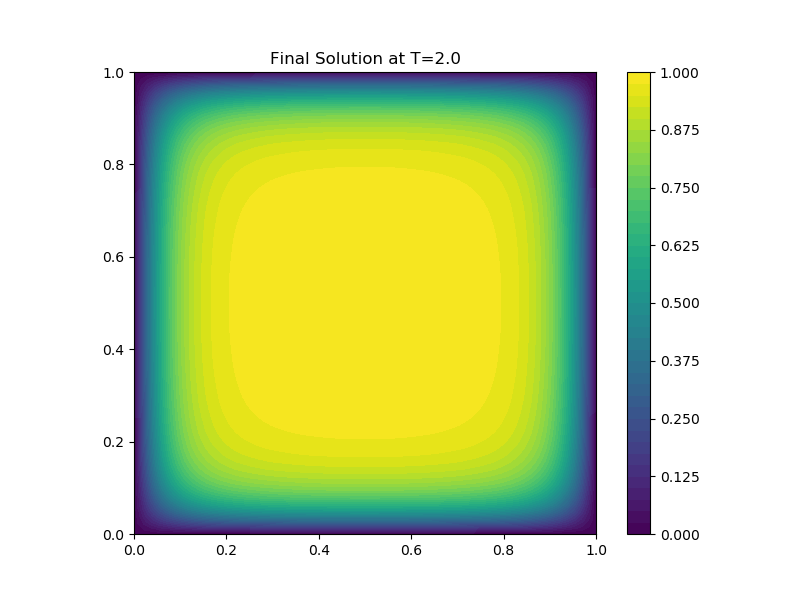
\includegraphics[width=0.7\textwidth]{final_solution.png}
    \caption{Final Solution at $T=2.0$}
    \label{fig:final}
\end{figure}

\section{Conclusion}
The reaction-diffusion equation was successfully derived and implemented in FEniCS. The results demonstrate the physical behavior of concentration spreading while being constrained by zero-value boundary conditions.

\end{document}
